\section{DSP Events}

The interface between the DSPs and the Event Bus provides low-latency
buffering of inbound and outbound events. Outbound events are
multiplexed between the two DSPs and are placed on the bus during the
appropriate stage in an Event Bus cycle. Only events which target a
given DSP are placed in its buffer.

Here is where we'd put an overview of the different sub-components,
and describe the input/output dichotomy

All parts of the event bus face challenges in switching from the CLK
to the SYSCLK domain and vice-versa.

\subsection{Event Bus Multiplexor}
      
      signals CEA and CEB for alternating DSPs A and B, alternating, via the ESEL signal
      
      Each DSP has a set of Address In (AI), Address Out (AO), Output Enable (OE), Data Out (DO), and Data In (DI) lines, as well as a signaling Clock Enable (CE). 

      The setting of MADDR : need some way to set wake-up signal, something something. 

      

\subsection{Event Outputs}

The event output subsystem uses the 16/32 bit dual-ported interface of
the BlockSelect+ RAM in the Spartan-3 to enable simultaneous read out
of the 16-bit data and 8 bit address during the event cycle, while
providing an easy 16-bit interface to the Parallel Port for the DSP.
\begin{figure}[h!]
\includegraphics[scale=0.8]{output.pdf}
\end{figure}



\subsubsection{Writing an Event to the output buffer}


The input to the Output Event Buffer is complex due to the desire to
preserve the 10-write-cycle length of an event write. A ROM maps the
latched \bus{ADDRL}{3:0} into the LSBs of
\bus{ADDRA}{9:0}, and the MSBs select the appropriate
buffer location through the Event Counter In
(\bus{ECNTIN}{5:0}).
        
The ROM mapping of addresses is necessary to have writes to locations
0x0, 0x1, and 0x2 map to the appropriate interleaved locations in the
buffer for read-out.  Each \signal{WE} assertion actually
triggers <emphasis>two</emphasis> writes of the RAM buffer, with the
ROM determining the necessary addresses and whether
\bus{DINL}{7:0} or \signal{DINL}{15:8} maps to the
low byte of \bus{DIA}{15:0}. An event write is considered
complete when the address 0x9 is written, thus incrementing
\bus{ECNTIN}{5:0}.
        

\begin{figure}[h!]
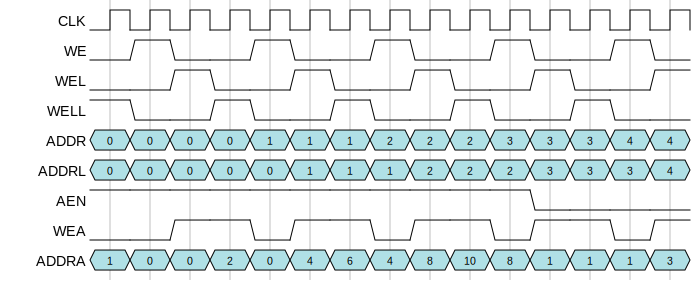
\includegraphics[scale=0.8]{write.timing.pdf}
\end{figure}                  
                
\subsubsection{Reading an event from the output buffer}
The output side of the buffer is in the \signal{SYSCLK}
domain, and uses the 32-bit wide interface of the BlockSelect+ RAM to
simultaneously read out the \signal{DATA} and
\signal{ADDR} portions of the event. The 3-bit
\bus{WCNT}{2:0} counter sequences through the individual
Event words, and the 6-bit \bus{ECNTOUT}{5:0} counter
selects the event from the buffer. These combine to form the address
input \bus{ADDRB}{8:0} to the RAM.
   
A complicated interplay of signals is necessary to guarantee that
\bus{EADDR}{7:0} and \signal{EDATA}{15:0} are valid
as soon as possible following the \signal{SYSCLK} edge that
registers \signal{ECE}. Thus, when not transmitting an Event,
the counters point to the first word of the next event in the buffer.

\begin{figure}[h!]
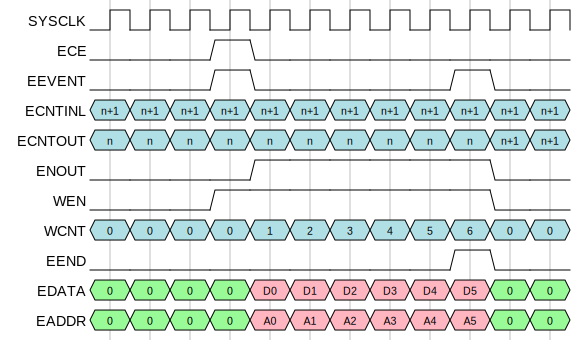
\includegraphics[scale=0.8]{output.timing.pdf}
\end{figure}                  

An example event output can be seen in . \bus{ECNTINL}{5:0}
is not equal to \signal{ECNTOUT}, indicating the presence of a
pending event. Note that \bus{ECNTINL}{5:0} would only be
incremented following the complete write of an event, thus there are
no potential timing conflicts. The simultaneous assertion of
\signal{EEVENT} and \signal{ECE} with events in the
buffer leads to the setting of \signal{ENOUT}.  This enables
the output muxes to drive the output data and address lines with the
real values from the event buffer.

\bus{WCNT}{2:0} is incremented while \signal{ENOUT}
is high <emphasis>and</emphasis> when \signal{EEVENT} and
\signal{ECE} are simultaneously asserted. Since the
BlockSelect+ RAM is synchronous (and thus the data output will follow
the input address by a clock signal) \bus{WCNT}{2:0} must
begin incrementing early.

\signal{EEND} goes high when \signal{WCNT}{2:0} equals
six, indicating the completion of an event write. This resets
\bus{ENOUT} and thus resets \bus{WCNT}{2:0}
while incrementing \bus{ECNTOUT}{5:0}.  
    

\subsubsection{Event Reader Stage}

Here's where we read the events off the Event Bus and potentially
store them if they are for us, that is, if the relevant ADDR bit is
set.


\begin{figure}[h!]
\includegraphics[scale=0.8]{reader.pdf}
\end{figure}
      
This is a challenge because we need to be able to read an event and
store it in our event buffer, <emphasis>even if</emphasis> we get two
events in a row. Thus, we use lots of pipelining.

To determine if an event is for us, we latch in each
\bus{EADDR}{7:0} byte, and use \bus{MADDR}{2:0}
to select the correct bit onto \signal{ADDRSEL}. The counter
\signal{CNT} is reset to zero in the cycle following
\signal{EVENTL} going high. \signal{SMINE} is set when
\signal{CNT} is equal to \bus{MADDR}{5:3}.
<emphasis>\signal{SMINE}'s set overrides its reset, which is
cleared on each cycle -- this is necessary to allow setting when the
relevant EADDR byte is at CNT=0. 

Each of \bus{D0}{15:0} through \bus{D5}{15:0} is
latched during the appropriate state in the Event, and the assertion
of \signal{LMINE} latches the corresponding values to the
registered \bus{D0L}{15:0} through
\bus{D5L}{15:0}, respectively. These are read
asynchronously via the outputs when \signal{MINE} is
eventually set.

\subsection{Event Inputs} 

\begin{figure}[h!]
\includegraphics[scale=0.8]{input.pdf}
\end{figure}

The transfer of the Events from the Event Bus to the DSP is relatively
simple compared to the other portions of the Event Subsystem. As the
Event Input system is in the \signal{SYSCLK} domain, we wait
for the falling edge of the \signal{EIN} via
\signal{EINDELTA}. Note that timing here is critical: A full
event cycle in the \signal{SYSCLK} domain takes at most 19
ticks in the \signal{CLK} domain.
      
The FSM waits for an assertion of \signal{EINDELTA} and then
checks for \signal{MINE} to be high, indicating that the
current event is targeted for this DSP. Then,
\bus{EDOUT}{7:0} is read to determine the CMD of the event.
A small subset of the potential events, related to resetting and
booting, are handled by the FPGA. All others are placed in a buffer
for the DSP.

\subsubsection{Mode Set}

When the Event's CMD is 0x01, we transition to <state>MODEEN</state>
and set the \signal{MODE} bit appropriately. Note that
\signal{MODE} can only be reset by the external
\signal{MODERST} line.

      
\subsubsection{DSP Reset}

The \signal{DSPRESET} signal is determined in a similar
manner, as the complement to the first data word of the Reset Event


\subsubsection{Boot RAM writes}


\bus{RAINCNT}{9:0} is first loaded with the target address
of the location in the boot RAM. The following four words are written
to that and the three subsequent addresses via
\bus{RDIN}{15:0} by incrementing
\bus{RAINCNT}{9:0} three times.


\subsubsection{Events targeted for the DSP}

All events not handled internally by the FPGA are placed in a
BlockSelect+ RAM circular buffer for later reading by the DSP. The
first word of each event is <emphasis>always</emphasis> written to the
current address pointed to by \bus{AEIN}{9:0}, regardless
of \signal{MINE} status. This should never be a problem as
\bus{AEIN}{9:0} should point to the next empty buffer
location at the start of each event read cycle. The next five words
are read and written sequentially into the buffer, with the low bits
of the address (\bus{AEIN}{2:0}) being controlled by the
FSM. The last stat ein the FSM incrmeents \bus{AEIN}{9:3},
positioning the system to write the next incoming event.

Readout is similar to other places in the FPGA, with
\signal{NEWEVENTS} signalling the presence of a non-empty
buffer. \bus{ADDR}{2:0} synchronously reads the relevant
words from the buffer, with a read of location 0x6 signalling the
completion of a read and thus incrementing
\bus{ADSPIN}{9:3}.

\subsection{Present concerns}
     1. For the event input stage, what kind of latch is SMINE? how is it possible for things to work when the MYADDR[5:3]=111, i.e.  in the last byte of the address?

